\chapter{Deep Learning For Simulation}
    Deep Learning, as a branch of Machine Learning, employs algorithms to process data and imitate the thinking process\cite{schmidhuber2015deep}, or to develop abstractions. Deep Learning (DL) uses layers of algorithms to process data, understand human speech, and visually recognize objects. Information is passed through each layer, with the output of the previous layer providing input for the next layer. The first layer in a network is called the input layer, while the last is called an output layer. All the layers between the two are referred to as hidden layers. Each layer is typically a simple, uniform algorithm containing one kind of activation function.  \\
    \begin{figure}[!ht]
        \centering
        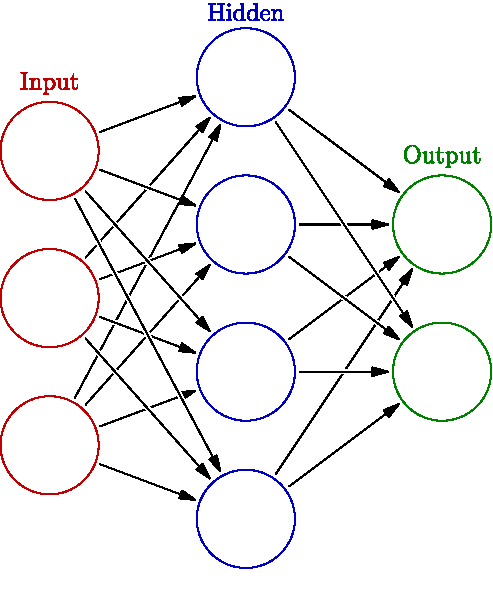
\includegraphics[scale = 0.5]{Figures/Colored_neural_network}
        \caption{visulization of one simple $3$-layers neural networks, including input layer, hidden layer and output layer, \textit{retrieved from Wikipedia}}
    \end{figure}

    With deep learning becoming more and more popular in many fields of researching, some classical methods can be replaced by deep learning. Many successful application of deep learning can be found in computer vision part, like image segmentation\cite{lecun2015deep},objection recognition\cite{he2016deep}. 

\section{Convolutional Neural Networks}
    An entire convolutional neural network consists of an input and output layer, as well as multiple hidden layers. Normally, the hidden layers consist of convolutional layer, pooling layers, fully conneted layers and normalization layers. \\

    Description of the process as a convolution in neural networks is by convention. Mathematically it is a cross-correlation rather than a convolution. This only has significance for the indices in the matrix, and thus which weights are placed at which index. 
    \subsection{Convolutional layers}
    Normal RGB images are represented by matrices containing color information in the form of Red-Gray-Blue color codes.

    \begin{figure}[!h]
        \centering
        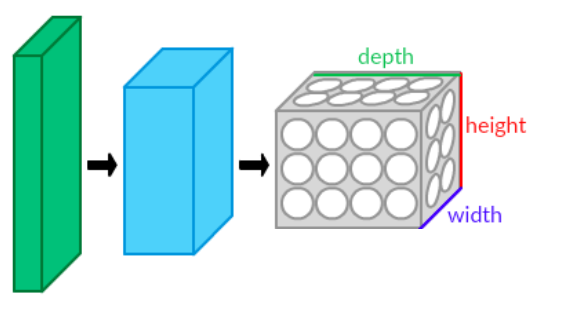
\includegraphics[scale = 0.3]{Figures/Conv_layers.png}
        \caption{Visualization of convolutions network, \textit{retrieved from Wikipedia}}
    \end{figure}

    \subsection{Pooling Layer}
    Pooling layers are also known as downsampling layers. A commonly used pooling is maxpooling(figure \ref{maxpooling}). The downsampled output is produced by taking the maxium input value within the kernel, resulting in output a decreased size. There are several other methods which are commonly used in neural networks, such as average pooling and L2-norm pooling. Average pooling was often used historically but has recently fallen out of favor compared to max pooling, which works better in practice\cite{scherer2010evaluation}.\\

    There are two important arguments for implementinf pooling layers,
    \begin{enumerate}
        \item Decreasing the number of weights.
        \item Decreasing the chance of overfitting the training data.
    \end{enumerate}
    \begin{figure}[!h]
        \centering
        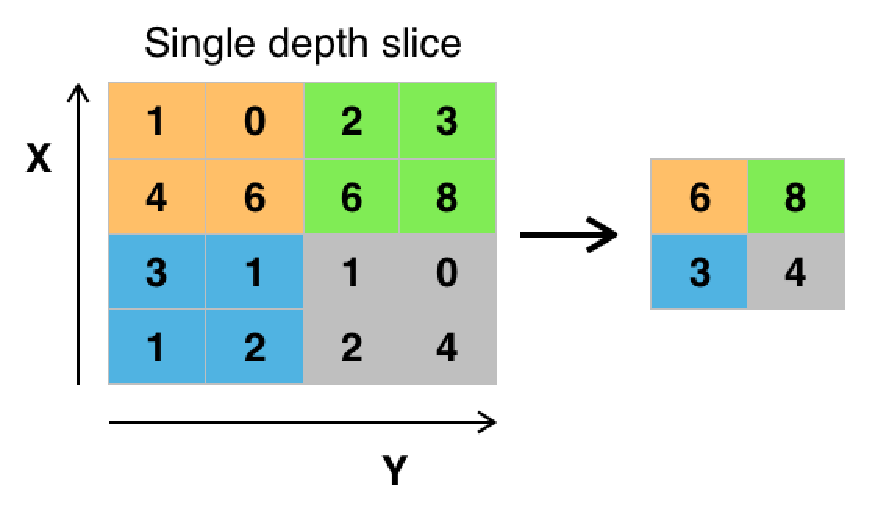
\includegraphics[scale=0.5]{Figures/Max_pooling.pdf}
        \caption{Maxpooling with a ($2\times 2$) kernel and stride $s=2$. Maxpooling layers reduce spatial dimension of the input \cite{li2015convolutional}}
        \label{maxpooling}
    \end{figure}

    \subsection{Fully connected Layer}
    Finally, after several convolutional and max pooling layers, the high-level reasoning in the neural network is done via fully connected layers. Neurons in a fully connected layer have connections to all activations in the previous layer, as seen in regular neural networks. Their activations can hence be computed with a matrix multiplication followed by a bias offset.

    \subsection{Overfitting}
    Overfitting is a problem that arises in neural network training. When a model is overfitted to the training data, it loses its capability of generalization. The model has learned the training data, including noise, in such a great extend that it has failed to capture underlying general information. CNNs have a large number of weights to be trained, therefore overfitting can occur due to training too few training examples. Dropout layers\cite{srivastava2014dropout} are a tool to prevent overfitting (Figure \ref{dropout}). In dropout, nodes and its connections are randomly dropped from the network. Dropout constrains the network adaptation to the training set, consequently it prevents that the weights are not too much fitted this data. The difference in performance between training data and validation data will decrease. Dropout layers are used during training only, not during validation or testing.

    \begin{figure}[!h]
        \centering
        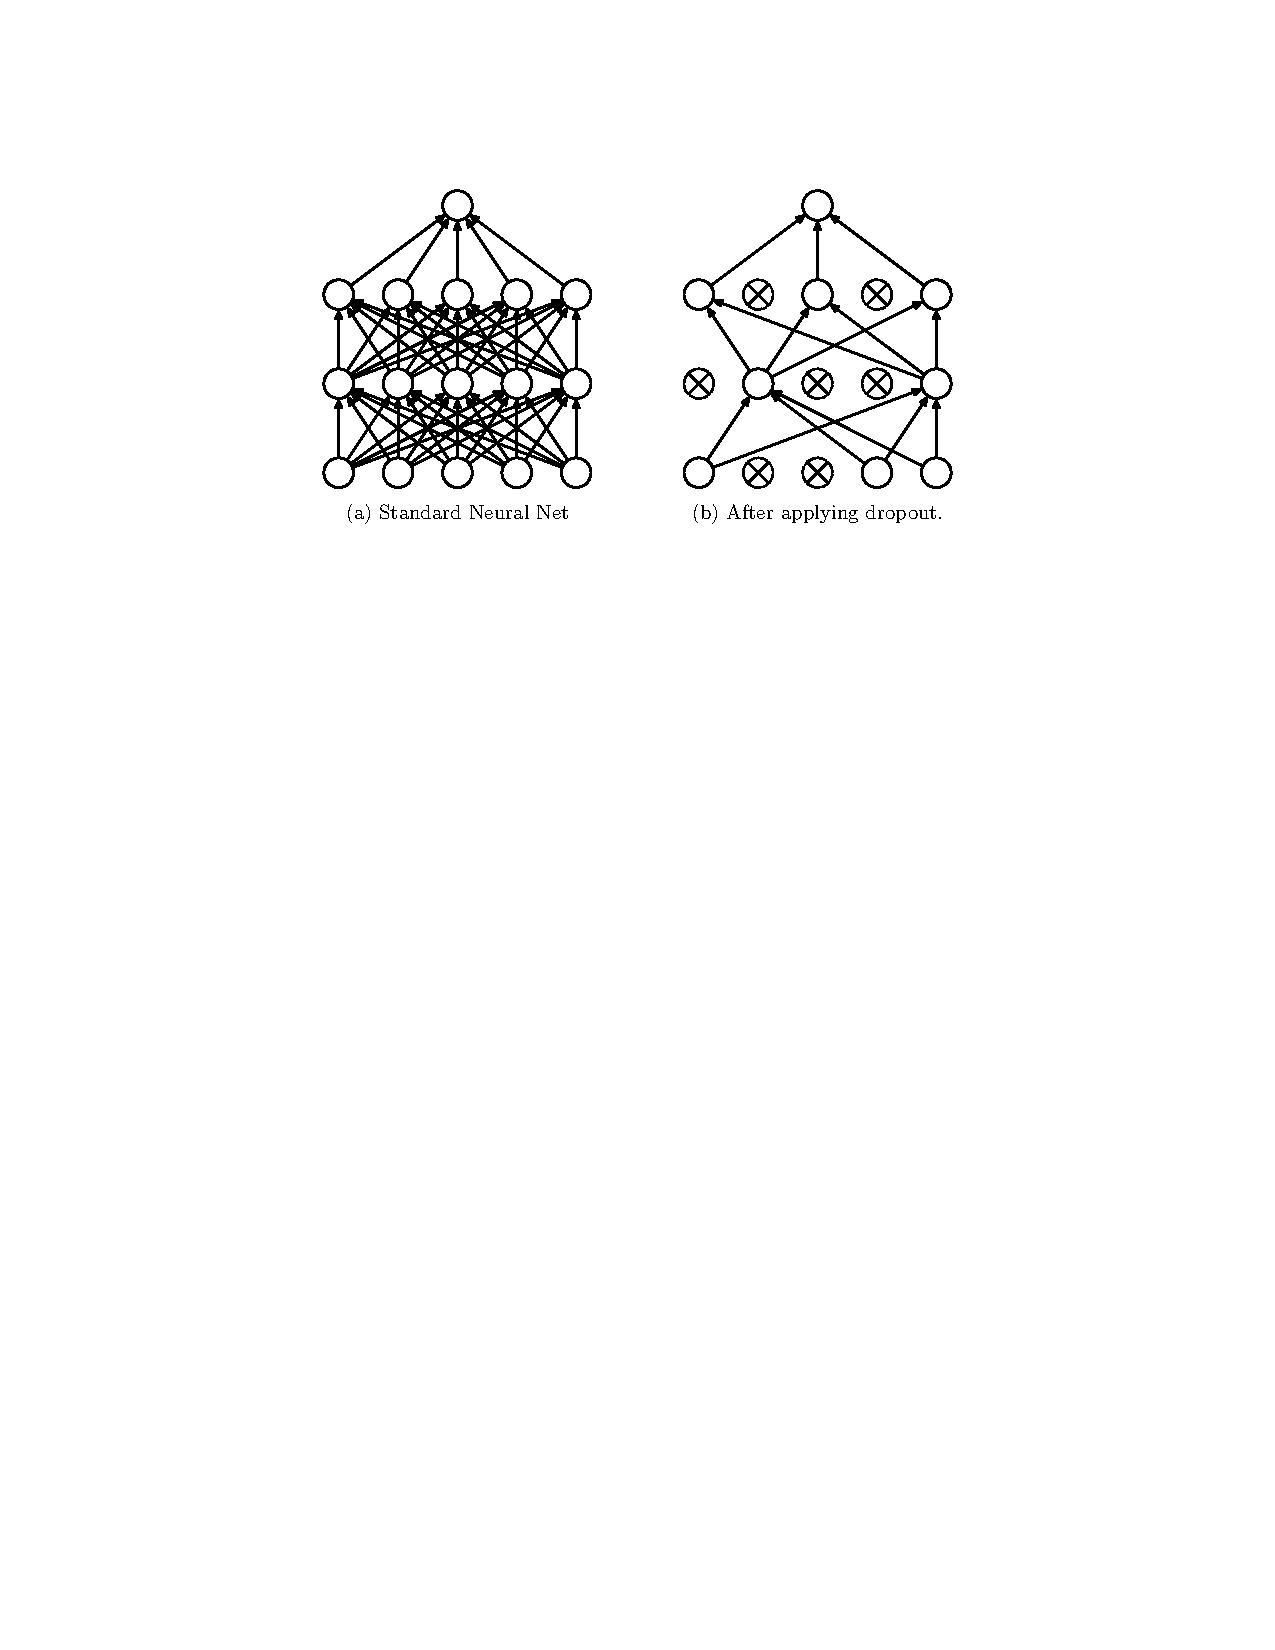
\includegraphics[scale=0.7]{Figures/dropout.pdf}
        \caption{A nerual network structure before and after applying dropout}
        \label{dropout}
    \end{figure}

    \subsection{Backpropagation}
    The CNN requires to adjust and update its kernel parameters, or weights, for the given training data. Backpropagation\cite{werbos1990backpropagation} is an efficient method for computing gradients required to perform gradient-based optimization of the weights in neural networks [19]. The specific combination of weights which minimize the loss function (or error function) is the solution of the optimization problem. The method requires the computation of the gradient of the error function at each iteration, therefore the loss function should be both continue and differentiable at all iteration steps.\\

    The initial weights of an untrained CNN are randomly chosen. Consequently before training, the neural network cannot make meaningful predictions for network input, as there is no relation between an image and the its labeled output yet. By exposing the network to a training data set, comprising images and their labeled outputs with correct classes, the weights are adjusted. Training is the adaptation of the weights in such way that the difference between desired output and network output is minimized, which means that the network is trained to find the right features required for classification. There are two computational phases in a neural network, the forward pass and the backward pass in which the weights are adapted.

    \subsubsection{Forward pass}
    An image is fed into a network. The first network layer outputs an activation map. Then, this activation map is the input to the first hidden layer, which computes another activation map. Using the values of this activation map as inputs to the second hidden layer, again another activation map is computed. Carrying out this process for every layer will eventually yield the network output.

    \subsubsection{Backward pass}
    In this phase the weights are updated by backpropagation. One epoch of backpropagation consists of multiple parts, usually multiple epochs are carried out for a training image:
    \begin{enumerate}
        \item \textbf{Loss Function} In forward pass, the inputs and desired outputs are presented. A pre-defined loss function $L$ is used to minimize the difference between the input and desired output. The goal is to adjust the weights so that the loss function value decreases, this is achieved by calculating the derivative with respect to the weights of the loss function.
        \item \textbf{Backward pass} During the backward pass, the weights that have contributed the most to the loss are chosen in order to adjust them so that the total loss decreases.
        \item \textbf{Weight update} In the final part all weights are updated in the negative direction of the loss function gradient.
    \end{enumerate}
    
    Therefore the core of the backpropagation problem is to compute the gradient of the loss function with respect to the network weights. Computing the partial derivative $\frac{\partial L}{\partial \omega}$ is essential(carried out in the backward pass) to minimize the loss function value. Stochastic Gradient Descent(SGD) is the most common way to optimize nerual networks.  

    \subsection{Stochastic Gradient Descent Variants}
    In both Gradient Descent (GD) and Stochastic Gradient Descent (SGD) parameters are updated according to an update rule to minimize a loss function in an iterative manner. Computing the exact gradient using GD in large datasets is expensive (GD is deterministic), as this method runs through all training samples to perform a single update for one iteration step. In Stochastic Gradient Descent (or on-line Gradient Descent) an approximation of the true gradient is computed. This is done by using only one or a subset of training samples for a parameter update. When using a subset of training samples, this method is called mini-batch SGD. \\

    SGD is a method to minize the loss function \(L(\theta)\)  parametrized by $\theta$. This is achieved by updating $\theta$ in the negative gradient direction of the loss function $\nabla_{\theta}L(\theta)$ with respect to the parameters, in order to decrease the loss function value. The learning rate $\eta$ determins the step size to get to the local or global minumum. 
    \begin{equation}
        \theta = \theta - \eta \nabla_{\theta}L(\theta)
    \end{equation}

    \subsubsection{Mini-batch Stochatic Gradient Descent}
    This method performs an update for every mini-batch of n training samples. Mini-batch SGD reduces the variance of the parameter updates. Larger mini-batches reduce the variance of SGD updates by taking the average of the gradients in the mini batch. This allows taking bigger step sizes. In the limit, if each batch contains one training sample, it is the same as regular SGD.

    

\section{CNN Constructure}
    \subsection{Convolutional layers}

    \subsection{Full-connected layers}

\section{Traing configuration}
    \subsection{Loss Function}

    \subsection{Optimizer(SGD)}

\section{Training Results}

\section{Simulation based on Trained model}